%%%%%%%%%%%%%%%%%%%%%%%%%%%%%%%%%%%%%%%%
\begin{figure*}[t]
    \centering
    \begin{subfigure}{0.44\textwidth}
        \centering
        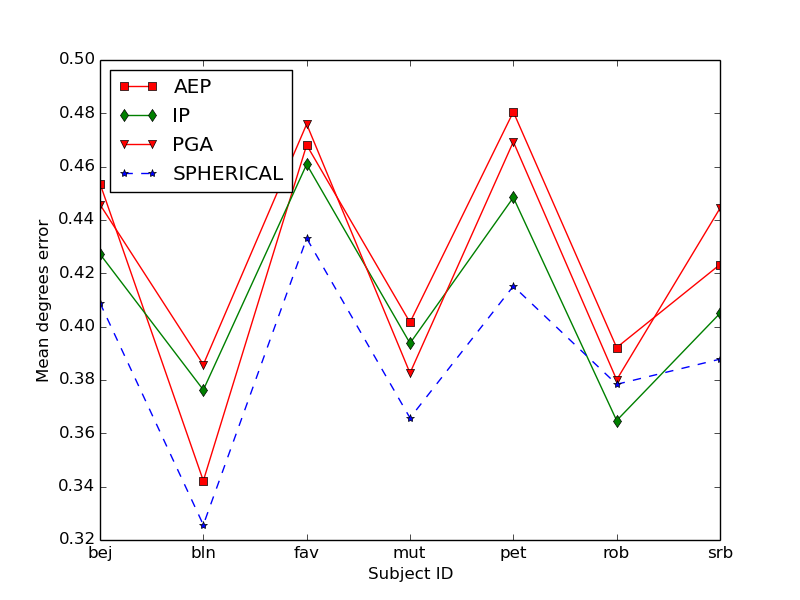
\includegraphics[width=\textwidth]{statistical_normals/images/gsfs_results/sfs-angle}
        \subcaption{The mean angular error per pixel between the ground truth 
                    normals and the reconstructions.}
\label{fig:sfs-angle}
    \end{subfigure}
    \;
    \begin{subfigure}{0.44\textwidth}
        \centering
        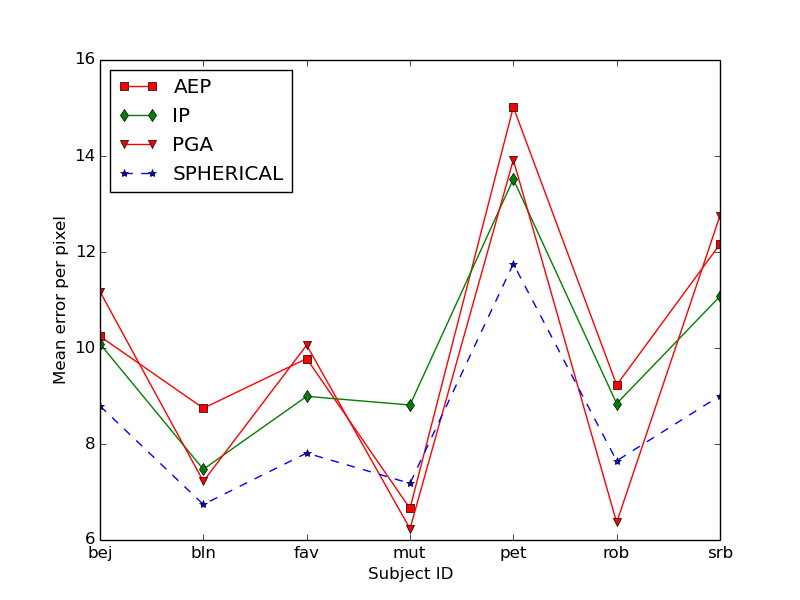
\includegraphics[width=\textwidth]{statistical_normals/images/gsfs_results/sfs-height}
        \subcaption{The mean error per pixel between the integrated shape and 
                    ground truth $z$-values.}
\label{fig:sfs-height}
    \end{subfigure}
    \caption{Quantitative results for shape-from-shading.}
\label{fig:sfs-results-quant}
\end{figure*}
%%%%%%%%%%%%%%%%%%%%%%%%%%%%%%%%%%%%%%%%
%%%%%%%%%%%%%%%%%%%%%%%%%%%%%%%%%%%%%%%%%%%%%%%%%%%%%%%%%%%%%%%%%%%%%%%%%%%%%%%%
\section{Experiments}\label{sec:experiments}
%%%%%%%%%%%%%%%%%%%%%%%%%%%%%%%%%%%%%%%%%%%%%%%%%%%%%%%%%%%%%%%%%%%%%%%%%%%%%%%%
We evaluated the performance of our kernel-base framework for component analysis 
on surface normals within three experimental setups. The experiments performed 
were chosen for two reasons: (1) We wanted to compare the reconstruction 
properties of all KPCA kernels from normals. (2) To compare the statistical 
prior of all KPCA kernels within shape-from-shading. 

We use the BU-4DFE dataset~\cite{RefWorks:104} and performed manual alignment 
of the scans. We also use FRGC v2 3D face database~\cite{RefWorks:251} to 
provide components of faces when operating within the GSFS framework. In each 
of the experiments, component analysis was performed as described in the 
previous section, and we refer to the AEP kernel as AEP, the PGA kernel as 
PGA, the inner product kernel as IP and the spherical kernel as SPHERICAL@.
%%%%%%%%%%%%%%%%%%%%%%%%%%%%%%%%%%%%%%%%%%%%%%%%%%%%%%%%%%%%%%%%%%%%%%%%%%%%%%%%
\subsection{Reconstruction Robustness}\label{subsec:Q}
%%%%%%%%%%%%%%%%%%%%%%%%%%%%%%%%%%%%%%%%%%%%%%%%%%%%%%%%%%%%%%%%%%%%%%%%%%%%%%%%
We considered a set of $108$ aligned 3D face scans from the BU-4DFE data-set, 
specifically for subject F001 with the emotion `Disgust'. These scans capture 
the face of F001 whilst displaying a posed example of the emotion where she 
transitions from neutral, to apex and back to neutral. We create two principal 
subspaces from this set of scans. In the first, which we call 
$\boldsymbol{U}_{noise-free}$, we simply perform KPCA on the scans for each of 
the considered kernel functions. In the second, which we call 
$\boldsymbol{U}_{noisy}$, we artificially occlude 20\% of the scan with a 
randomly generated patch of normals. We occlude a total of 20\% of the images 
in the set before creating the noisy principal subspace. The performance 
measure we use to evaluate each kernel is independent of the feature-space, 
instead computing the total similarity between the principal components of 
$\boldsymbol{U}_{noise-free}$ and $\boldsymbol{U}_{noisy}$. Formally, the 
performance measure is defined as 
$Q = \sum_{i=1}^k \sum_{j=1}^k \cos(\alpha_{ij})$ where $\alpha_{ij}$ is the 
angle between each of the $k$ eigenvectors defined by
 $\boldsymbol{U}_{noise-free}$ and $\boldsymbol{U}_{noisy}$. 

The ideal value of $Q$ would be $k$, the number of coincident spaces, and is 
shown in Figure~\ref{fig:Q} as the black diamond-marked line. Figure~\ref{fig:Q} 
shows the mean value over 10 different sets of randomly placed normals for
 F001-Disgust. In Figure~\ref{fig:Q} we can clearly see that AEP and SPHERICAL 
 are the most robust to the noisy subspace.
%%%%%%%%%%%%%%%%%%%%%%%%%%%%%%%%%%%%%%%%%%%%%%%%%%%%%%%%%%%%%%%%%%%%%%%%%%%%%%%%
\subsection{Reconstruction Evaluation}
%%%%%%%%%%%%%%%%%%%%%%%%%%%%%%%%%%%%%%%%%%%%%%%%%%%%%%%%%%%%%%%%%%%%%%%%%%%%%%%%
We used the same experimental setup as in Section~\ref{subsec:Q} to produce 
$\boldsymbol{U}_{noisy}$ for each kernel. For every corrupted image in the 
training set we then projected it into the appropriate feature-space and 
reconstructed it with an increasing number of principal components from
 $\boldsymbol{U}_{noisy}$:
%%%%%%%%%%%%%%%%%%%%
\begin{equation}\label{eq:xtilde}
    \tilde{\boldsymbol{X}} = \phi^{-1} \left( \boldsymbol{U}_{noisy} \; {\boldsymbol{U}_{noisy}}^T \phi(\boldsymbol{X}) \right)
\end{equation}
%%%%%%%%%%%%%%%%%%%%
where $\phi$ and $\phi^{-1}$ are different for each method, as defined in 
Section~\ref{sec:subspace-analysis}. After reconstruction we project the 
feature vector back in to the input space of surface normals and re-normalised 
each normal. Finally, our evaluation metric was defined as the total angular
 error between the reconstructed and the ground truth normals.

The mean value of the total angular error for the first 10 principal 
components is given in Figure~\ref{fig:reconstruction-error}. Here we can 
see that SPHERICAL outperforms the other techniques by a large margin.
%%%%%%%%%%%%%%%%%%%%%%%%%%%%%%%%%%%%%%%%%%%%%%%%%%%%%%%%%%%%%%%%%%%%%%%%%%%%%%%%
\subsection{Shape-from-shading}
%%%%%%%%%%%%%%%%%%%%%%%%%%%%%%%%%%%%%%%%%%%%%%%%%%%%%%%%%%%%%%%%%%%%%%%%%%%%%%%%
Images from the Photoface Database~\cite{RefWorks:293} were used to provide a 
ground truth model. We used the photometric stereo algorithm presented by 
\citet{RefWorks:108} in order to reconstruct a set of normals. 
We consider the normals computed by photometric stereo as ground truth due to 
their relative accuracy over SFS@.

Seven people from the data-set were chosen at random. The four images of each 
person were manually aligned and photometric stereo was performed to produce a
set of ground truth normals per subject. Then, one of the images was chosen 
and the GSFS framework described by \citet{RefWorks:86,RefWorks:90} 
was performed to reconstruct normals. The set of priors used to guide the GSFS 
was generated according to the KPCA framework described 
\cref{sec:kpca,sec:subspace-analysis} and the training set used was provided by 
building a model from the FRGC v2 dataset~\cite{RefWorks:251}.

The model was built from the Spring 2003 subset of the FRGC database after 
applying some simple pre-processing in the form of hole filling and a median 
filter. A needle-map was created from the depthmap. Each image in the FRGC 
database was manually annotated with 68 points, as were the images from the 
Photoface database. We performed a thin-plate spline warp to each needle-map 
of the FRGC database to warp the needle-map into the reference space defined 
by the Photoface image landmarks. Due to the different reference spaces, a 
separate set of warped needle-maps was built for each input image. Statistical 
models were then created from the warped needle-maps according to the kernels 
described in Section~\ref{sec:subspace-analysis}.

To produce Figure~\ref{fig:sfs-results} we applied the procedure described in 
Algorithm~\ref{alg:gsfs} with each of the kernels, AEP, PGA, IP and SPHERICAL 
in turn. Once a set of best-fit normals was recovered from GSFS, we applied 
the integration method of \citet{RefWorks:99}. 
Therefore, \cref{fig:sfs-results} shows the surfaces reconstructed 
after integration. \cref{fig:sfs-angle} shows the mean angular error 
per pixel. Here we see that SPHERICAL consistently outperforms the other 
kernels for angular error accuracy. SPHERICAL also performs well in terms of 
the mean height error between the photometric stereo reconstruction and the 
GSFS result as shown in \cref{fig:sfs-height}. \cref{fig:sfs-results} 
shows that the GSFS produces realistic results within this setting for all kernels.
%%%%%%%%%%%%%%%%%%%%%%%%%%%%%%%%%%%%%%%%
\begin{figure*}
    \centering
    \sfsimgsalltop{bej} \\
    \sfsimgsall{bln} \\
    % \sfsimgsall{fav} \\
    % \sfsimgsall{mut} \\
    % \sfsimgsall{pet} \\
    % \sfsimgsall{rob} \\
    % \sfsimgsall{srb}
    \caption{Each row represents a subject. From top to bottom the subject 
             identifiers are `bej', `bln', `fav', `mut', `pet', `rob', `srb'}
\label{fig:sfs-results}
\end{figure*}
%%%%%%%%%%%%%%%%%%%%%%%%%%%%%%%%%%%%%%%%
%%%%%%%%%%%%%%%%%%%%%%%%%%%%%%%%%%%%%%%%%%%%%%%%%%%%%%%%%%%%%%%%%%%%%%%%%%%%%%%%
\subsection{Comparison to other SFS techniques}\label{subsec:sfs-compare}
%%%%%%%%%%%%%%%%%%%%%%%%%%%%%%%%%%%%%%%%%%%%%%%%%%%%%%%%%%%%%%%%%%%%%%%%%%%%%%%%
Barron and Malik provide a state-of-the-art SFS technique in 
\cite{RefWorks:225,RefWorks:224} which they call shape, illumination and 
reflectance from shading (SIRFS). We attempted to reconstruct the same input 
images given in the first column of Figure~\ref{fig:sfs-results} using the 
default parameters provided by the authors. An example of the output produced 
by the SIRFS algorithm is given in the final column of Figure~\ref{fig:sfs-results}. 
As we can see, the lack of prior knowledge produces a result that is clearly 
less accurate than the proposed statistical models of normals.

\citet{RefWorks:226} propose a methodology to recover 
facial shape from single images using a single template shape. Unfortunately, 
we were unable to reproduce their results and received no response when 
contacting them. However, \cref{fig:celebrities} shows that when running 
GSFS on a subset of the same images of celebrities reported in~\cite{RefWorks:226}, 
we can achieve comparable results. For example, in \cref{fig:samuel-beckett-wrinkles} 
we can see that GSFS is also capable of recovering the wrinkles from an input image. 
The results in \cref{fig:celebrities} follow a similar methodology to the 
Photoface database where the light direction is estimated as in~\cite{RefWorks:226} 
and the kernel used is SPHERICAL@.
%%%%%%%%%%%%%%%%%%%%%%%%%%%%%%%%%%%%%%%%
\begin{figure}
    \centering
    \begin{subfigure}{0.32\textwidth}
        \centering
        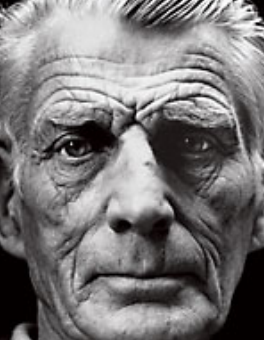
\includegraphics[width=0.8\textwidth]{statistical_normals/images/gsfs_results/celebrities/samuel_beckett.png}
\label{fig:samuel-beckett-input}
    \end{subfigure}
    \begin{subfigure}{0.32\textwidth}
        \centering
        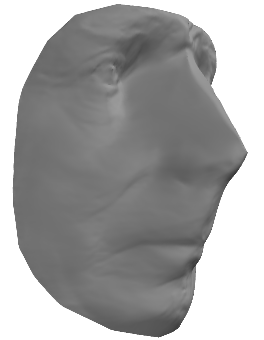
\includegraphics[width=0.8\textwidth]{statistical_normals/images/gsfs_results/celebrities/samuel_beckett_spherical.png}
\label{fig:samuel-beckett-no-texture}
    \end{subfigure}
    \begin{subfigure}{0.32\textwidth}
        \centering
        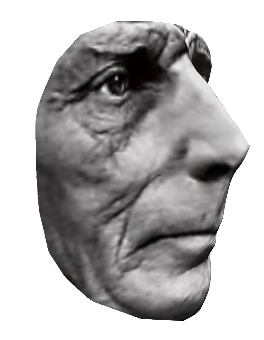
\includegraphics[width=0.8\textwidth]{statistical_normals/images/gsfs_results/celebrities/samuel_beckett_spherical_texture.png}
\label{fig:samuel-beckett-textured}
    \end{subfigure}
    \\
    \begin{subfigure}{0.32\textwidth}
        \centering
        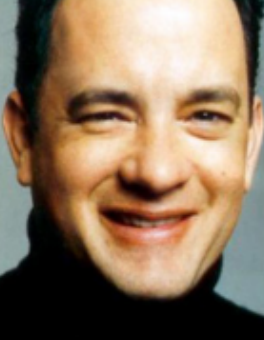
\includegraphics[width=0.8\textwidth]{statistical_normals/images/gsfs_results/celebrities/tom_hanks.png}
\label{fig:tom-hanks-input}
    \end{subfigure}
    \begin{subfigure}{0.32\textwidth}
        \centering
        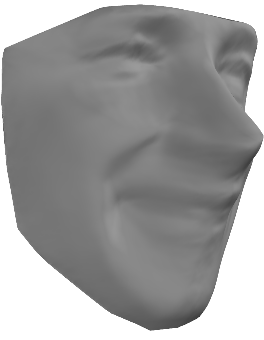
\includegraphics[width=0.8\textwidth]{statistical_normals/images/gsfs_results/celebrities/tom_hanks_spherical.png}
\label{fig:tom-hanks-no-texture}
    \end{subfigure}
    \begin{subfigure}{0.32\textwidth}
        \centering
        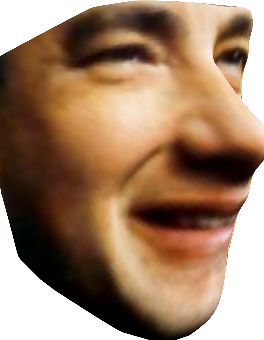
\includegraphics[width=0.8\textwidth]{statistical_normals/images/gsfs_results/celebrities/tom_hanks_spherical_texture.png}
\label{fig:tom-hanks-textured}
    \end{subfigure}
    \caption{The result of the GSFS algorithm on images of celebrities taken
             from~\cite{RefWorks:226} using the SPHERICAL kernel.}
\label{fig:celebrities}
\end{figure}
%%%%%%%%%%%%%%%%%%%%%%%%%%%%%%%%%%%%%%%%
%%%%%%%%%%%%%%%%%%%%%%%%%%%%%%%%%%%%%%%%
\begin{figure}
    \centering
    \begin{subfigure}{0.4\textwidth}
        \centering
        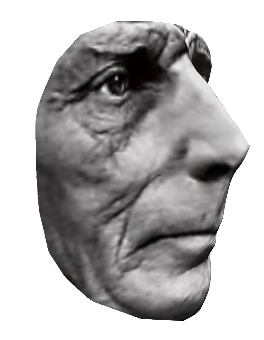
\includegraphics[width=\textwidth]{statistical_normals/images/gsfs_results/celebrities/samuel_beckett_spherical_texture.png}
    \end{subfigure}
    \begin{subfigure}{0.4\textwidth}
        \centering
        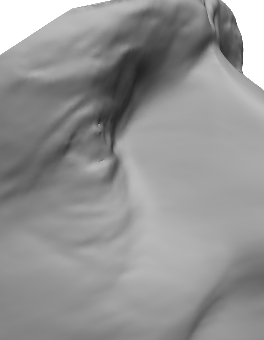
\includegraphics[width=\textwidth]{statistical_normals/images/gsfs_results/celebrities/samuel_beckett_spherical_wrinkles.png}
    \end{subfigure}
    \caption{A close up of the wrinkles recovered when running GSFS on the 
             image of Samuel Beckett shown in Figure~\ref{fig:celebrities}}
\label{fig:samuel-beckett-wrinkles}
\end{figure}
%%%%%%%%%%%%%%%%%%%%%%%%%%%%%%%%%%%%%%%%
